\documentclass[tikz]{standalone}
\usepackage[sfdefault,light]{roboto}
\usetikzlibrary{shapes, arrows, positioning, backgrounds}
\tikzset{every picture/.style={/utils/exec={\sffamily}}}
\begin{document}
    \begin{tikzpicture} [
			every node/.style={align=center, draw=none, fill=none, minimum width=2cm},
			legend/.style={font=\small},
		]
			\node (client) [legend] {Client};
			\node (serveur) [legend, right=6cm of client] {Serveur};
			\node (ordiClient) [above=0.4cm of client] {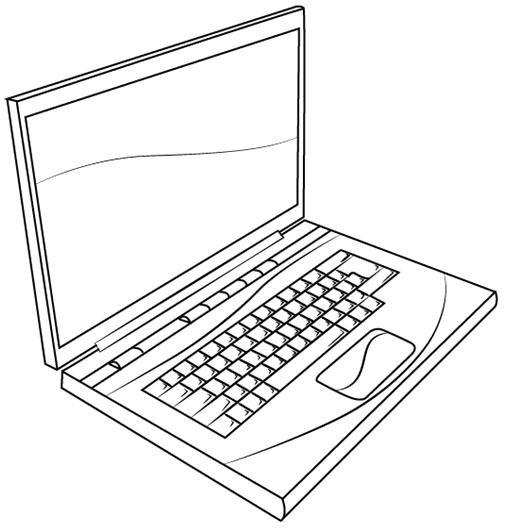
\includegraphics[width=20mm]{images/pc.png}};
			\node (ordiServeur) [above=0.4cm of serveur]  {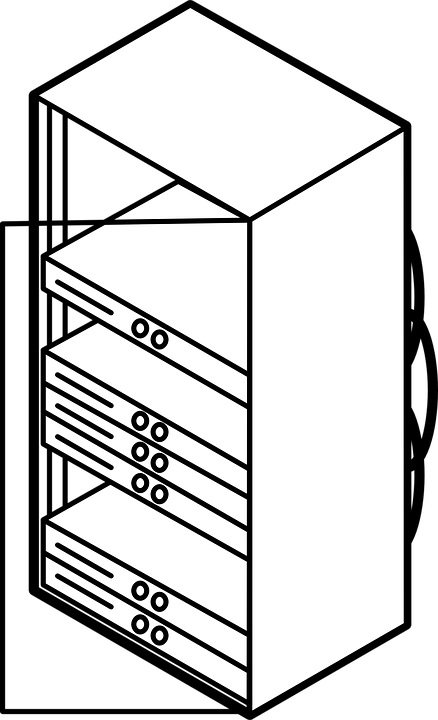
\includegraphics[width=16mm]{images/server.png}};
			\node [legend, above=0.5cm of ordiClient] {
				\texttt{3. Visualisation}
			};
			\path[-latex,thick] (ordiClient.20) edge node [legend,above] {
				\texttt{1. Requête:} \\
				\texttt{demande d'un fichier index.html}
			} (ordiServeur.west|-ordiClient.20);
			\path[latex-,thick] (ordiClient.-20) edge node [legend,below] {
				\texttt{2. Réponse:} \\
				\texttt{le fichier index.html demandé}
			} (ordiServeur.west|-ordiClient.-20);
			\path[-latex,thick] (ordiClient) edge [looseness=2, out=100, in=160] (ordiClient);
		\end{tikzpicture}
\end{document}